\subsection{IPTV}

As previously mentioned, the test environments didn’t have an \gls{iptv} subscription of the \gls{isp}, but information the data collected indicates how it could be properly configured. Although problems like the \gls{sip} keep-alive packets wouldn’t be detected.

\begin{figure}[h]
    \centering
    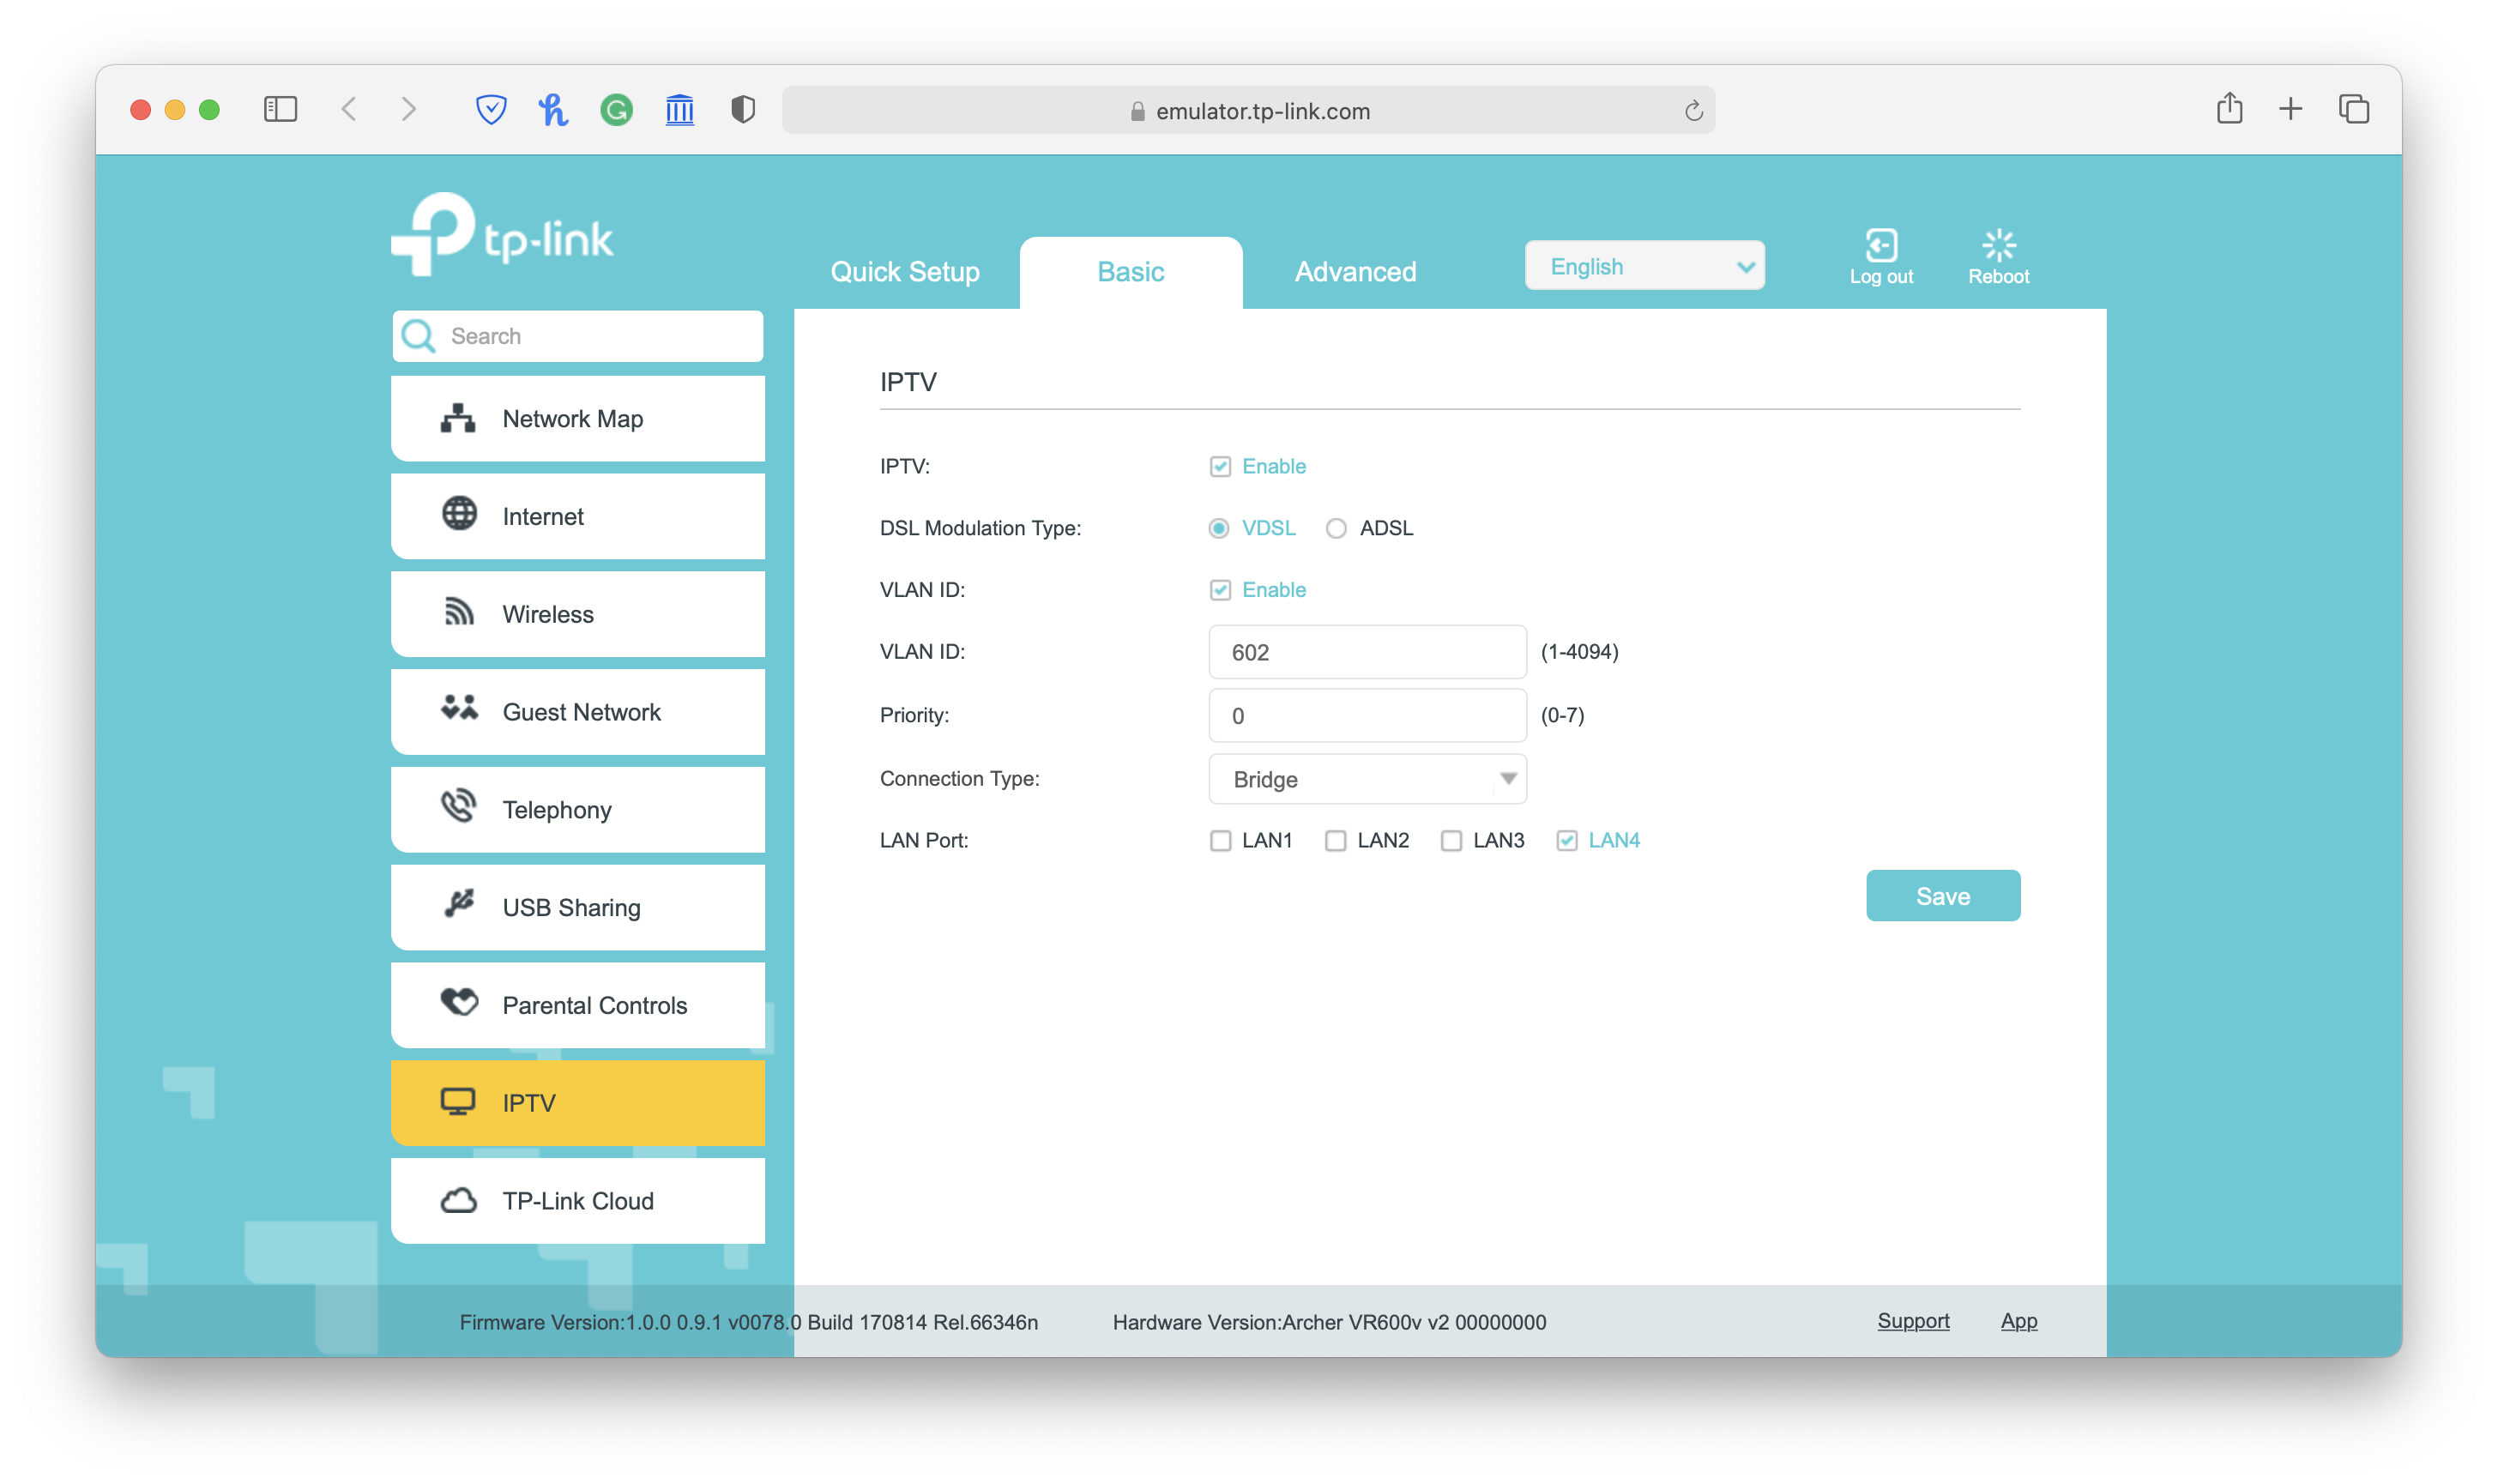
\includegraphics[width=\linewidth]{contents/substituting-the-isp-cpe/iptv/basic-iptv.png}
    \caption{\gls{iptv} Settings of the \gls{crg}s}
    \label{figure:crgs_iptv}
\end{figure}

The \gls{iptv} traffic is routed through a third network. This can be configured on the basic section of the \gls{http} Management Interface, as shown on Figure \ref{figure:crgs_iptv}. \gls{iptv} is enabled, the \gls{vlan} \gls{id} is set 602, and the Connection Type kept as Bridge. The set-top box provided by the \gls{isp} is connected to a \gls{lan} port of the residential gateway through an Ethernet cable. That specific \gls{lan} port must be checked on the configuration page of \gls{iptv}, allowing the \gls{stb} to access the correct \gls{vlan}.

This should be enough to have the \gls{iptv} service properly working, unfortunately it wasn’t verifiable and additional tweaking may be required.

\FloatBarrier
